\chapter{色覚多様性と作図}
\label{chap:color}

\section{色覚多様性とは}

「色覚多様性」や「色覚特性」という言葉を聞いたことがあるでしょうか。もし聞いたことがなくても、「色覚異常」「色盲」「色弱」という言葉であれば知っているかもしれません\footnote{これら言葉の使用の是非についてはこの文章の範囲を超えるので論じませんが、本章では「色覚多様性」という表現で統一します。左利きの人や AB 型の人ををわざわざ「利き手異常」「血液型異常」と呼ばないように、「異常」のような言葉の使用を避ける人が多いということは知っておいてください。}。人間の色覚は人によって異なり、あなたの目で見ている色の見え方が他の人とは異なる場合があります。このような多様性を、色覚多様性と言います。

人によって異なると言っても、人間の色覚はいくつかの種類に分類されます。血液型が人によって違ったり、利き手の左右が違ったりと同様です。例えば日本人男性の場合、その約5\%は赤と緑の色の差を区別しにくいという色覚を持っていると言われています。日本人女性であれば0.2\%、白人男性であれば8\%程度とも言われています。

図\ref{fig_color_line1}は 2 つの関数を色の違いのみで描いたものです。両方とも実線を使っていますが、$\sin(x)$ は赤、$\cos(x)$ は緑を使用しています。あなたが運よく多数派の(「正常」と呼ばれる)色覚特性を持つのであれば、これら 2 つの関数の区別は問題なく行えるでしょう。しかし赤と緑の区別が困難な人には、同じものが図\ref{fig_color_line2}のように見えている可能性があります。

% \begin{figure}
%   \centering
%   \subfigure[]{%
%     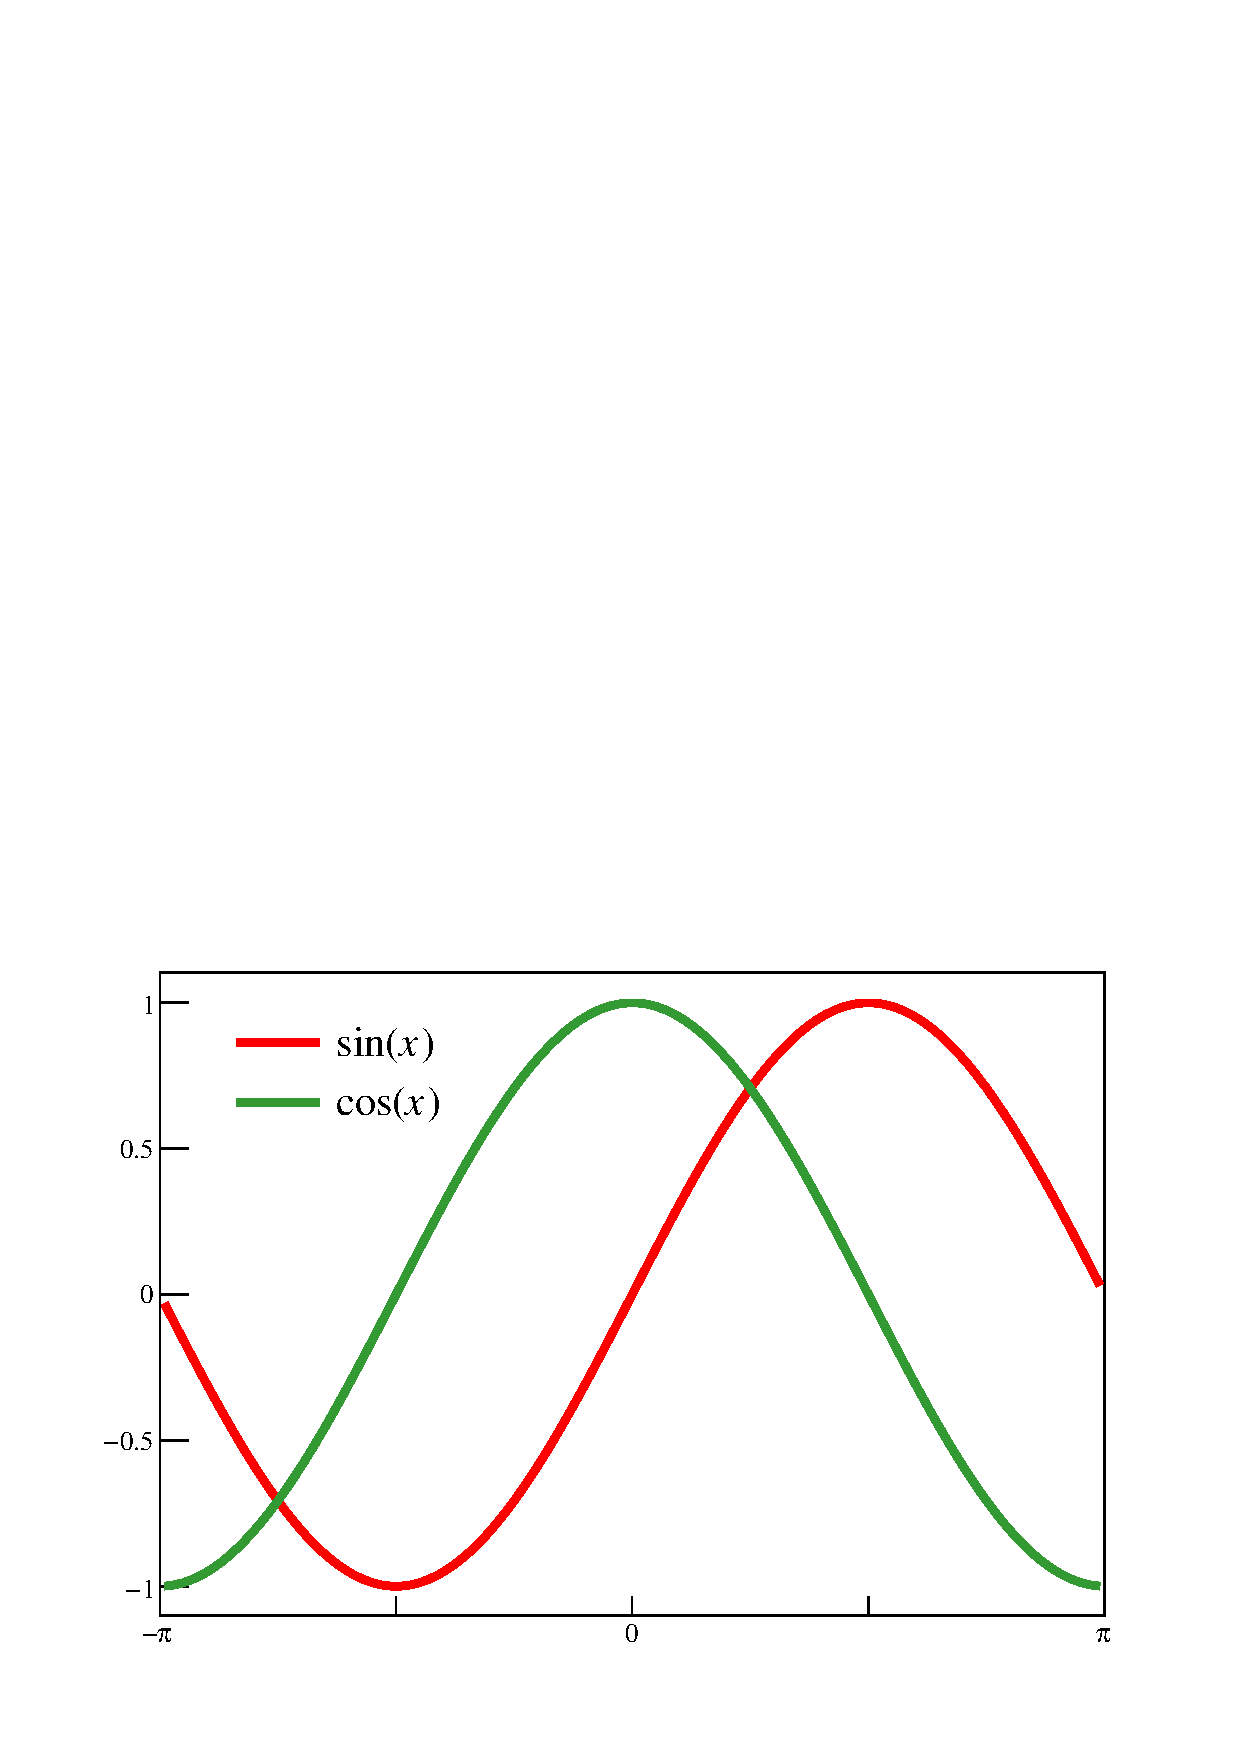
\includegraphics[width=.5\textwidth,clip]{fig/color_line1.pdf}%
%     \label{fig_color_line1}%
%   }%
%   \subfigure[]{%
%     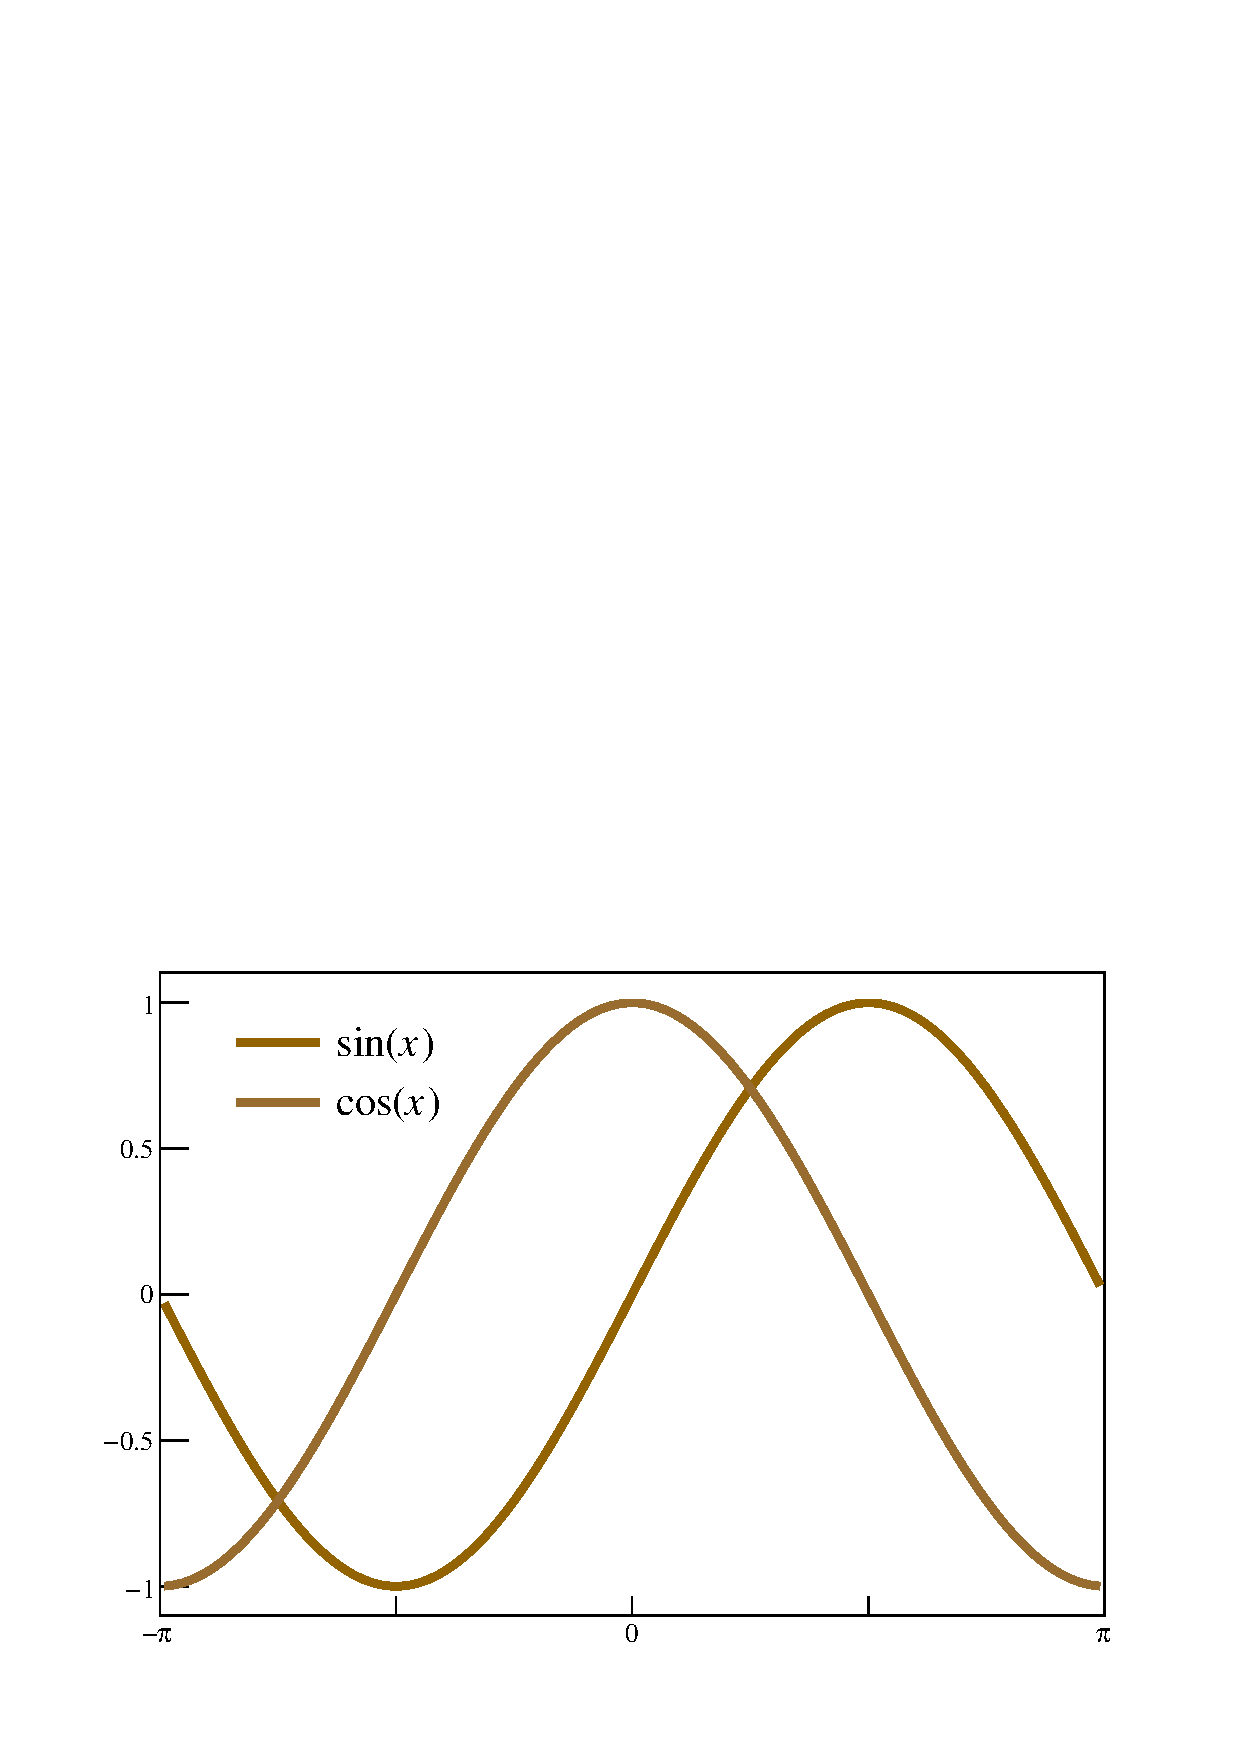
\includegraphics[width=.5\textwidth,clip]{fig/color_line2.pdf}%
%     \label{fig_color_line2}%
%   }
%   \caption[色覚特性による図の見え方の違い]{色覚特性による図の見え方の違い。(a) 「正常」とされる場合の人は、この赤と緑の区別がつく。(b) 赤と緑の区別がつきにくい色覚特性を持つ人には、このように見える(シミュレーション)。}
% \end{figure}

\section{色覚多様性を配慮した作図}

\subsection{線種の変更}
それでは、図\ref{fig_color_line1}に示したような2つの関数を誰にでも区別できるようにするには、どのようにすれば良いでしょうか。曲線や直線を使用している図の場合、線種を変更するのが一般的に行われる手法です。図\ref{fig_color_line3}では色の違いに加えて線種の違いを加えました。これであれば色の違いが分からなくても、図\ref{fig_color_line4}のように2つの関数を区別できるようになります。一度に表示する線の数が多い場合、実線、破線、点線、一点鎖線、太線、細線などと使い分けましょう。

% \begin{figure}
%   \centering
%   \subfigure[]{%
%     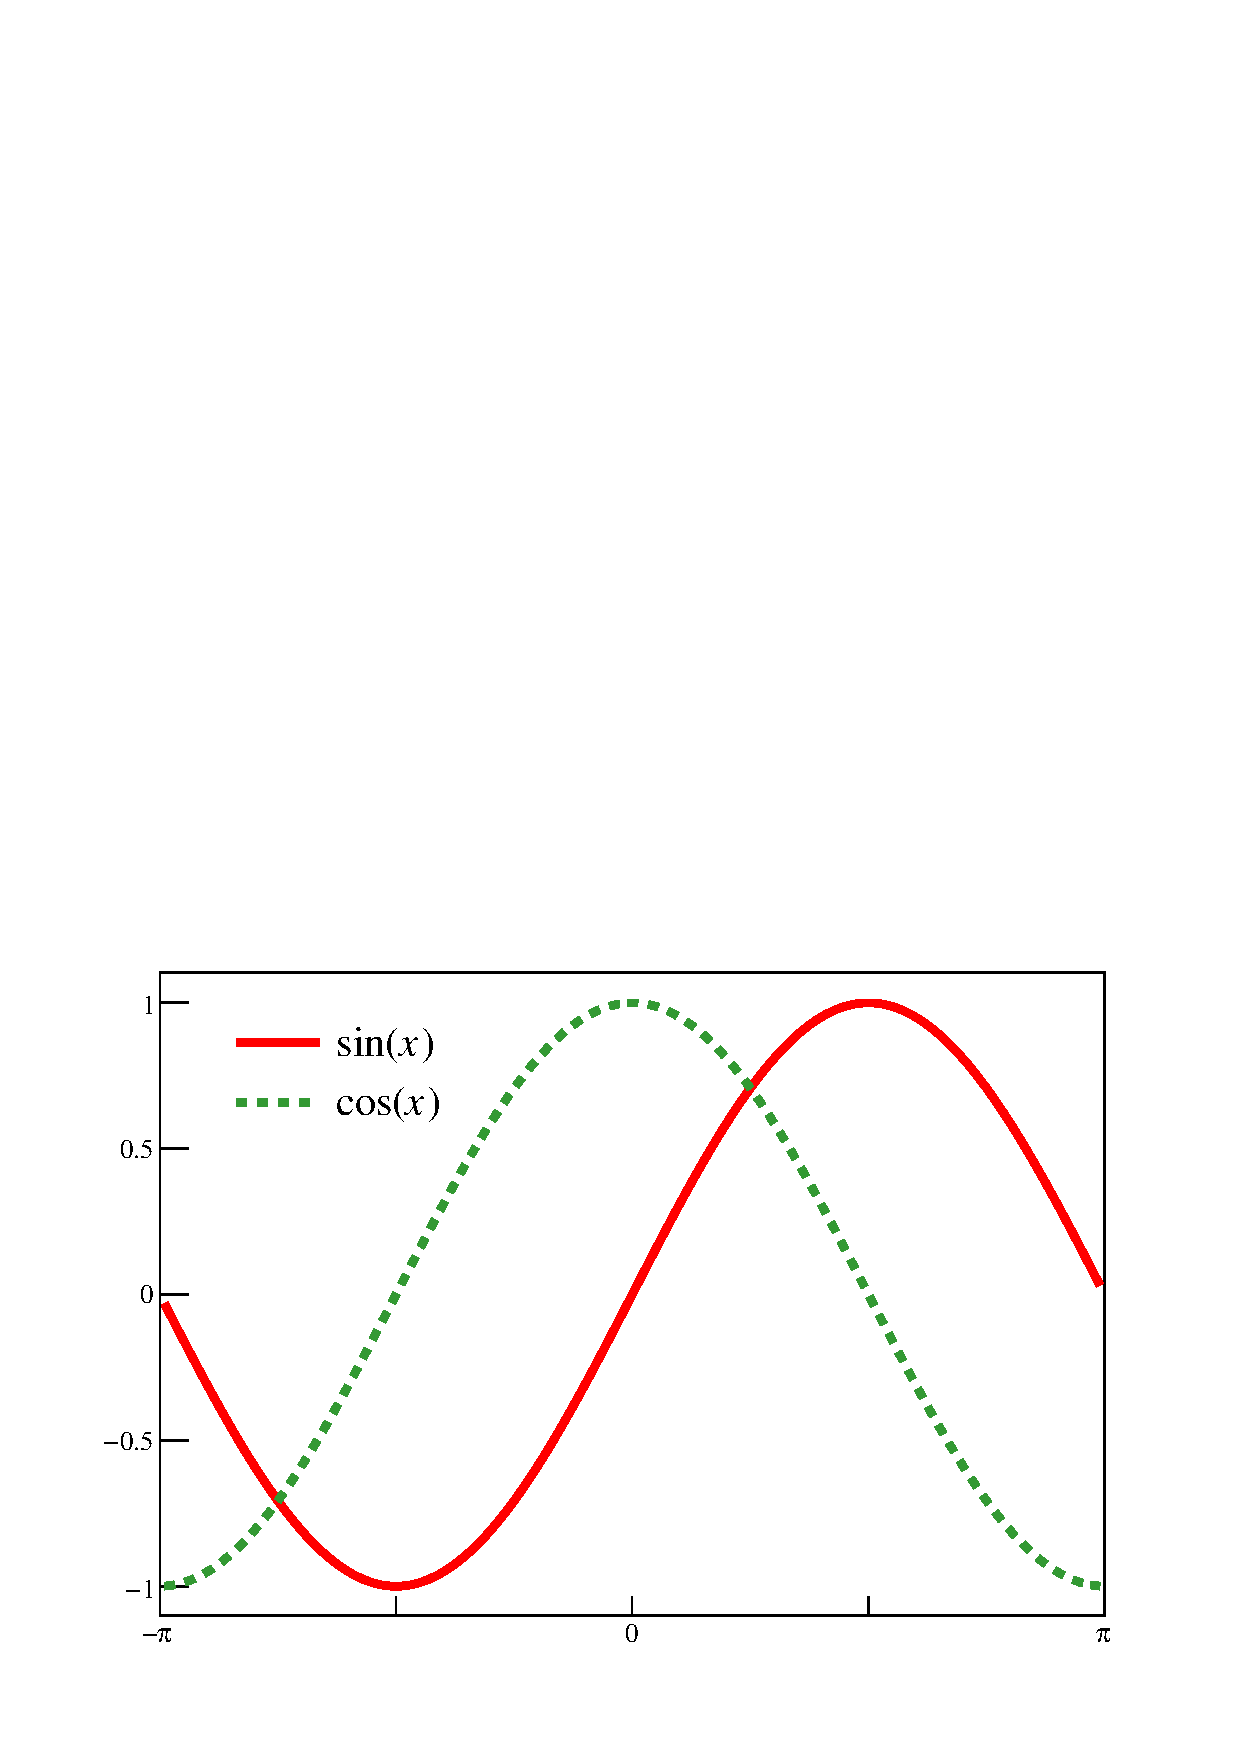
\includegraphics[width=.5\textwidth,clip]{fig/color_line3.pdf}%
%     \label{fig_color_line3}%
%   }%
%   \subfigure[]{%
%     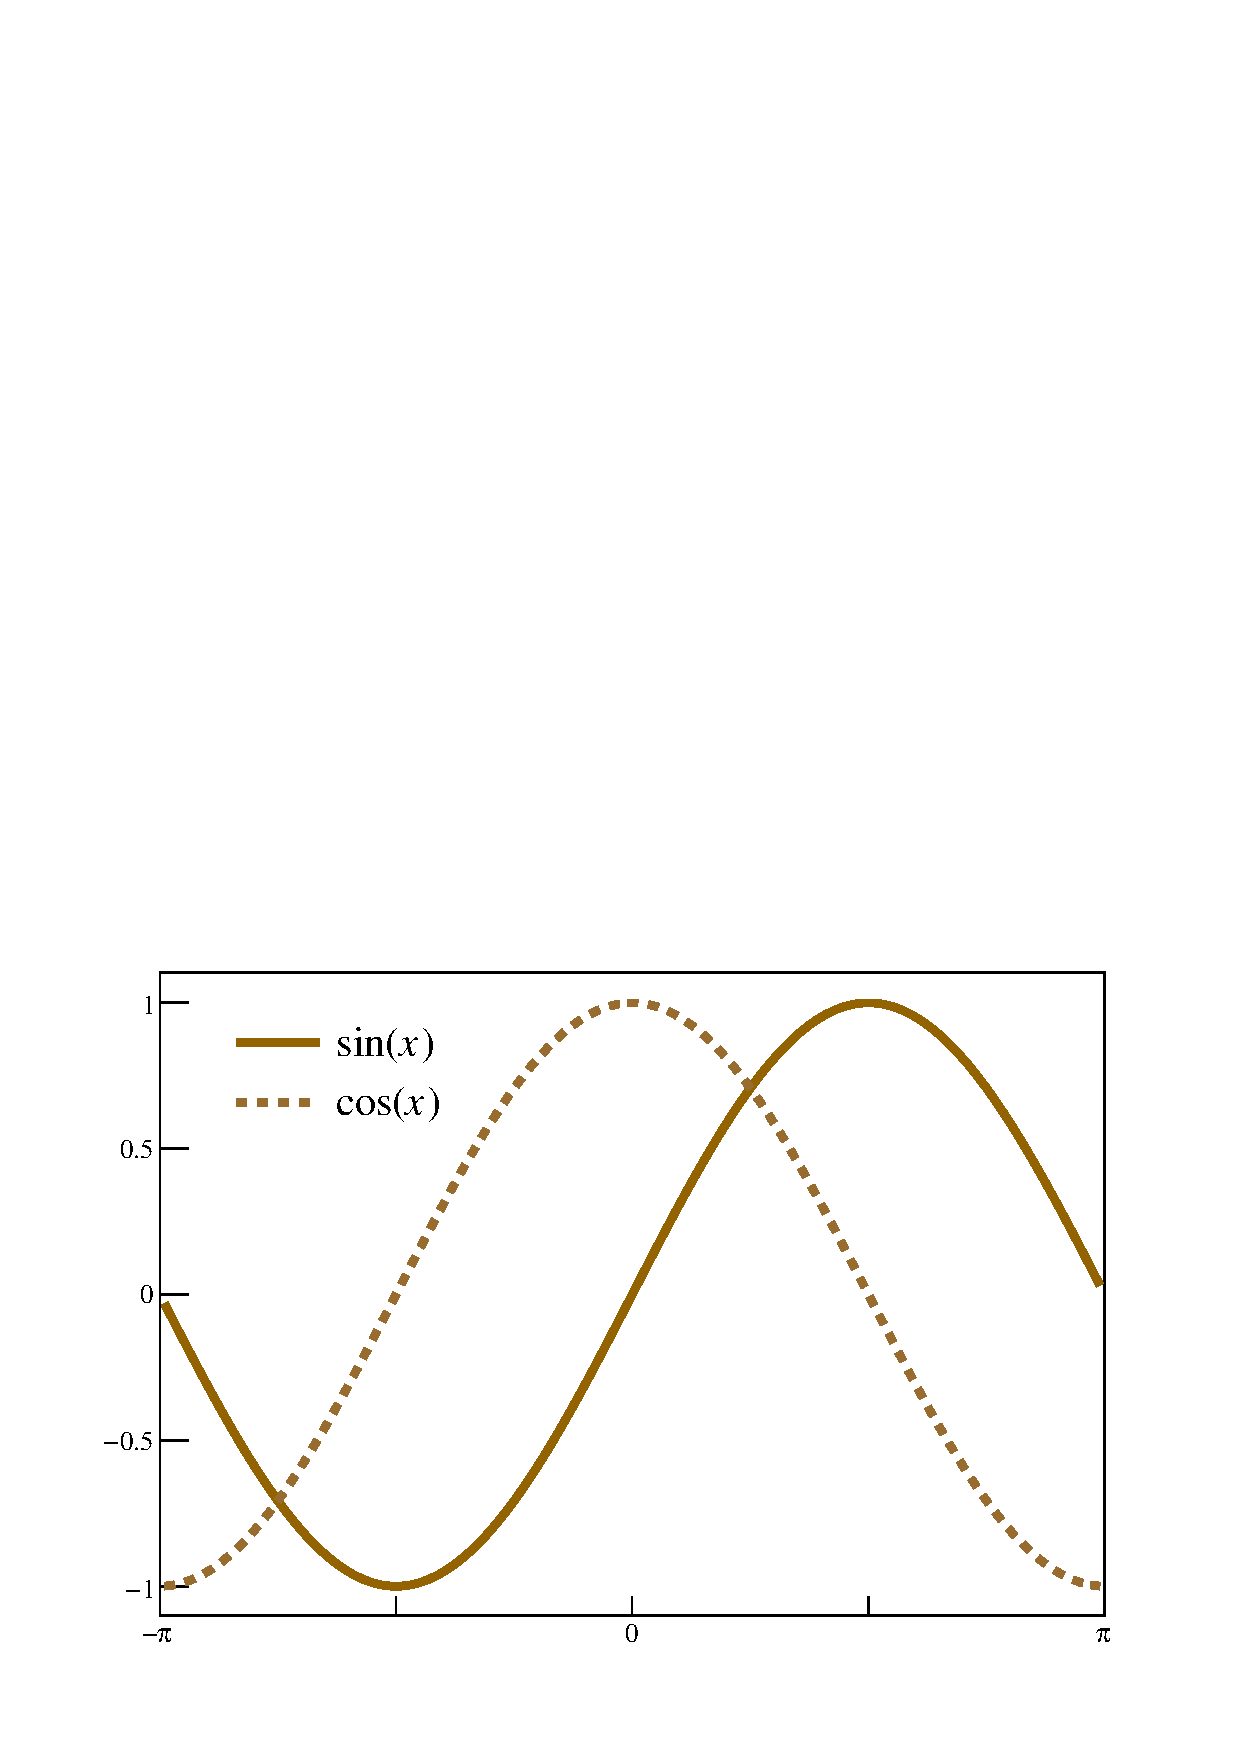
\includegraphics[width=.5\textwidth,clip]{fig/color_line4.pdf}%
%     \label{fig_color_line4}%
%   }
%   \caption[色覚特性を考慮した作図例]{色覚特性を考慮した作図例。(a) 色の違いに加えて、線種も変更した。(b) 赤と緑の区別ができなくても、線種によって区別が可能。}
% \end{figure}

\subsection{マーカー形状の変更}

散布図のようにデータ点を表示する場合、印(マーカー)の形状を変更します。赤も緑も青もよく使う色ですので図\ref{fig_color_marker1}のような図は修論でも学会でもよく見かけます。しかし、例えば赤と緑の区別がつかない色覚特性の場合、これは図\ref{fig_color_marker2}のように化けます。最悪ですね、なにも区別できなくなります。

これはマーカーの形状を変更することで、図\ref{fig_color_marker4}のように容易に区別が着くようになります。測定値を折れ線グラフで結ぶような場合は、さらに折れ線の線種も変更することでより区別しやすくなる場合があります。

% \begin{figure}
%   \centering
%   \subfigure[]{%
%     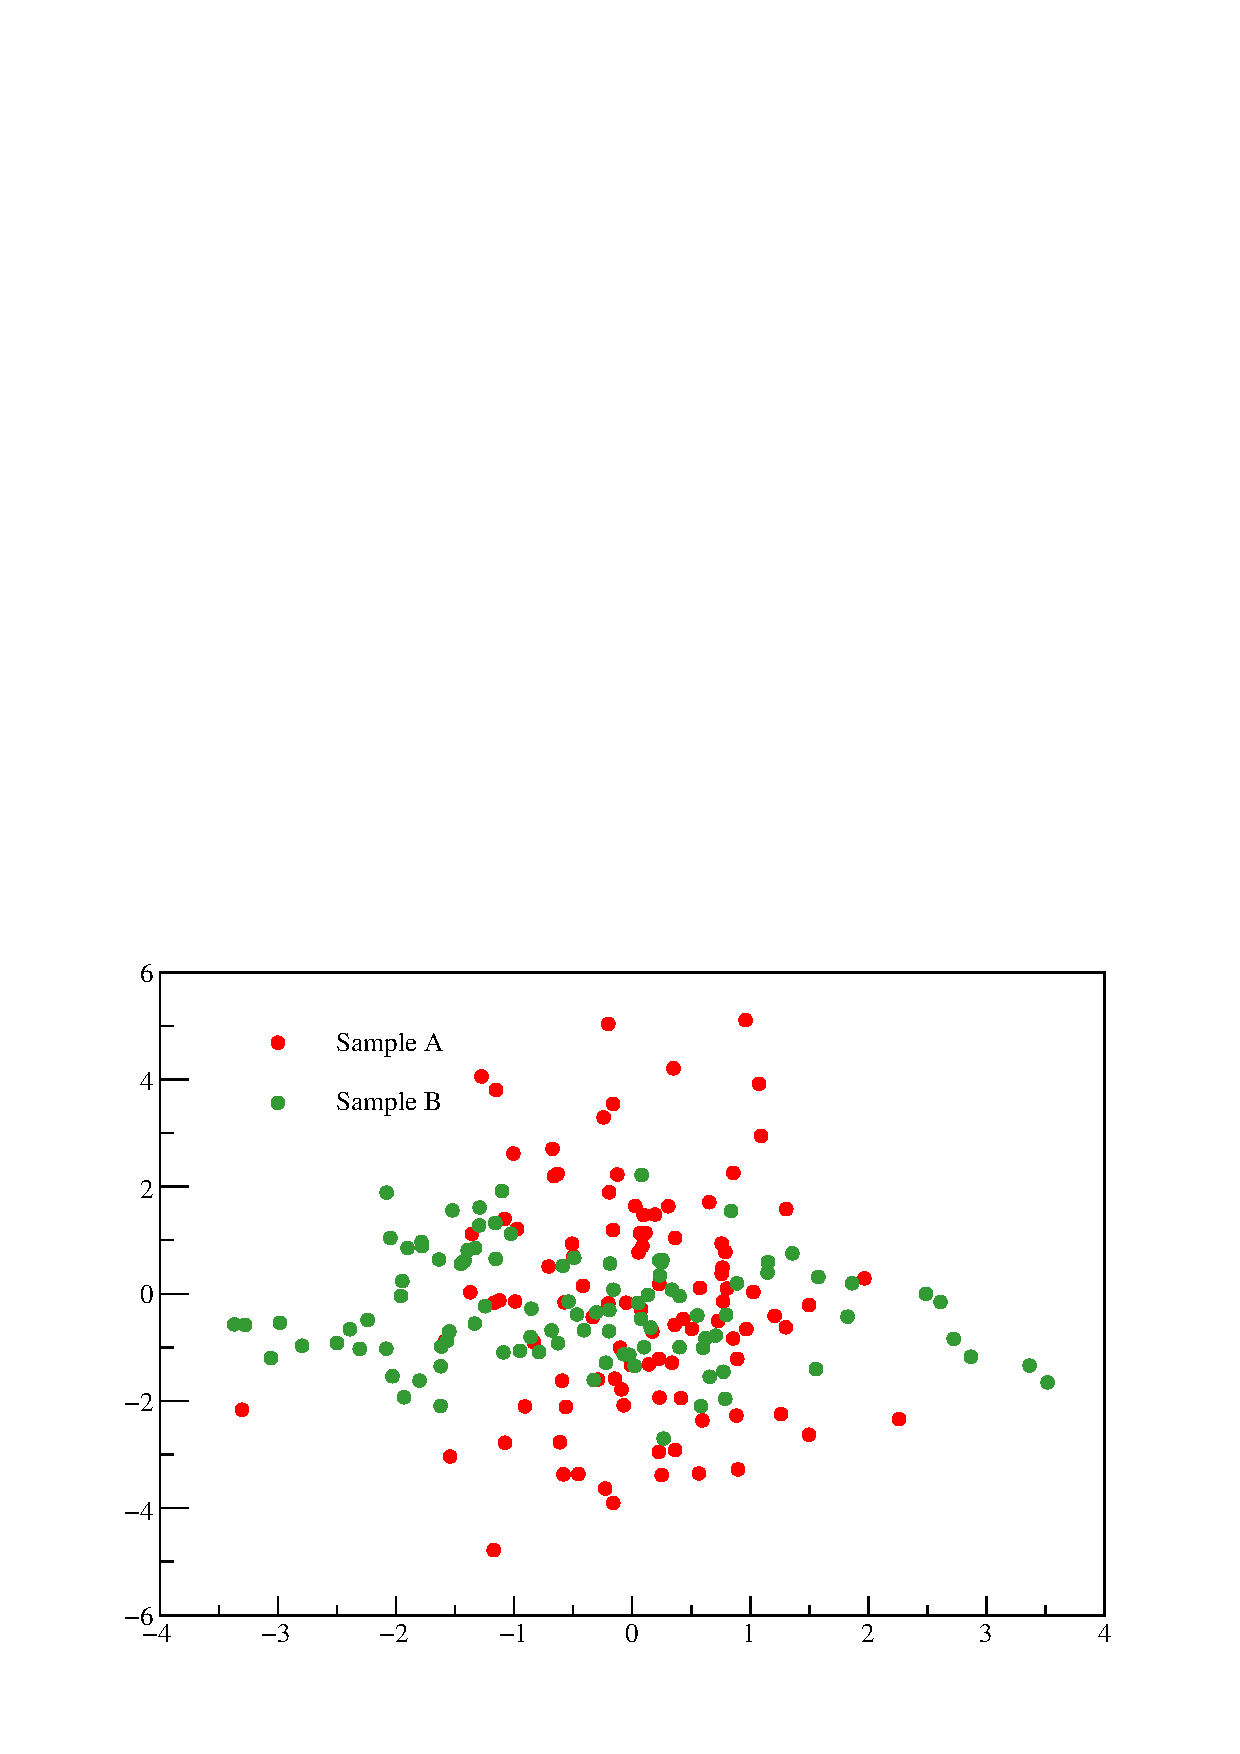
\includegraphics[width=.5\textwidth,clip]{fig/color_marker1.pdf}%
%     \label{fig_color_marker1}%
%   }%
%   \subfigure[]{%
%     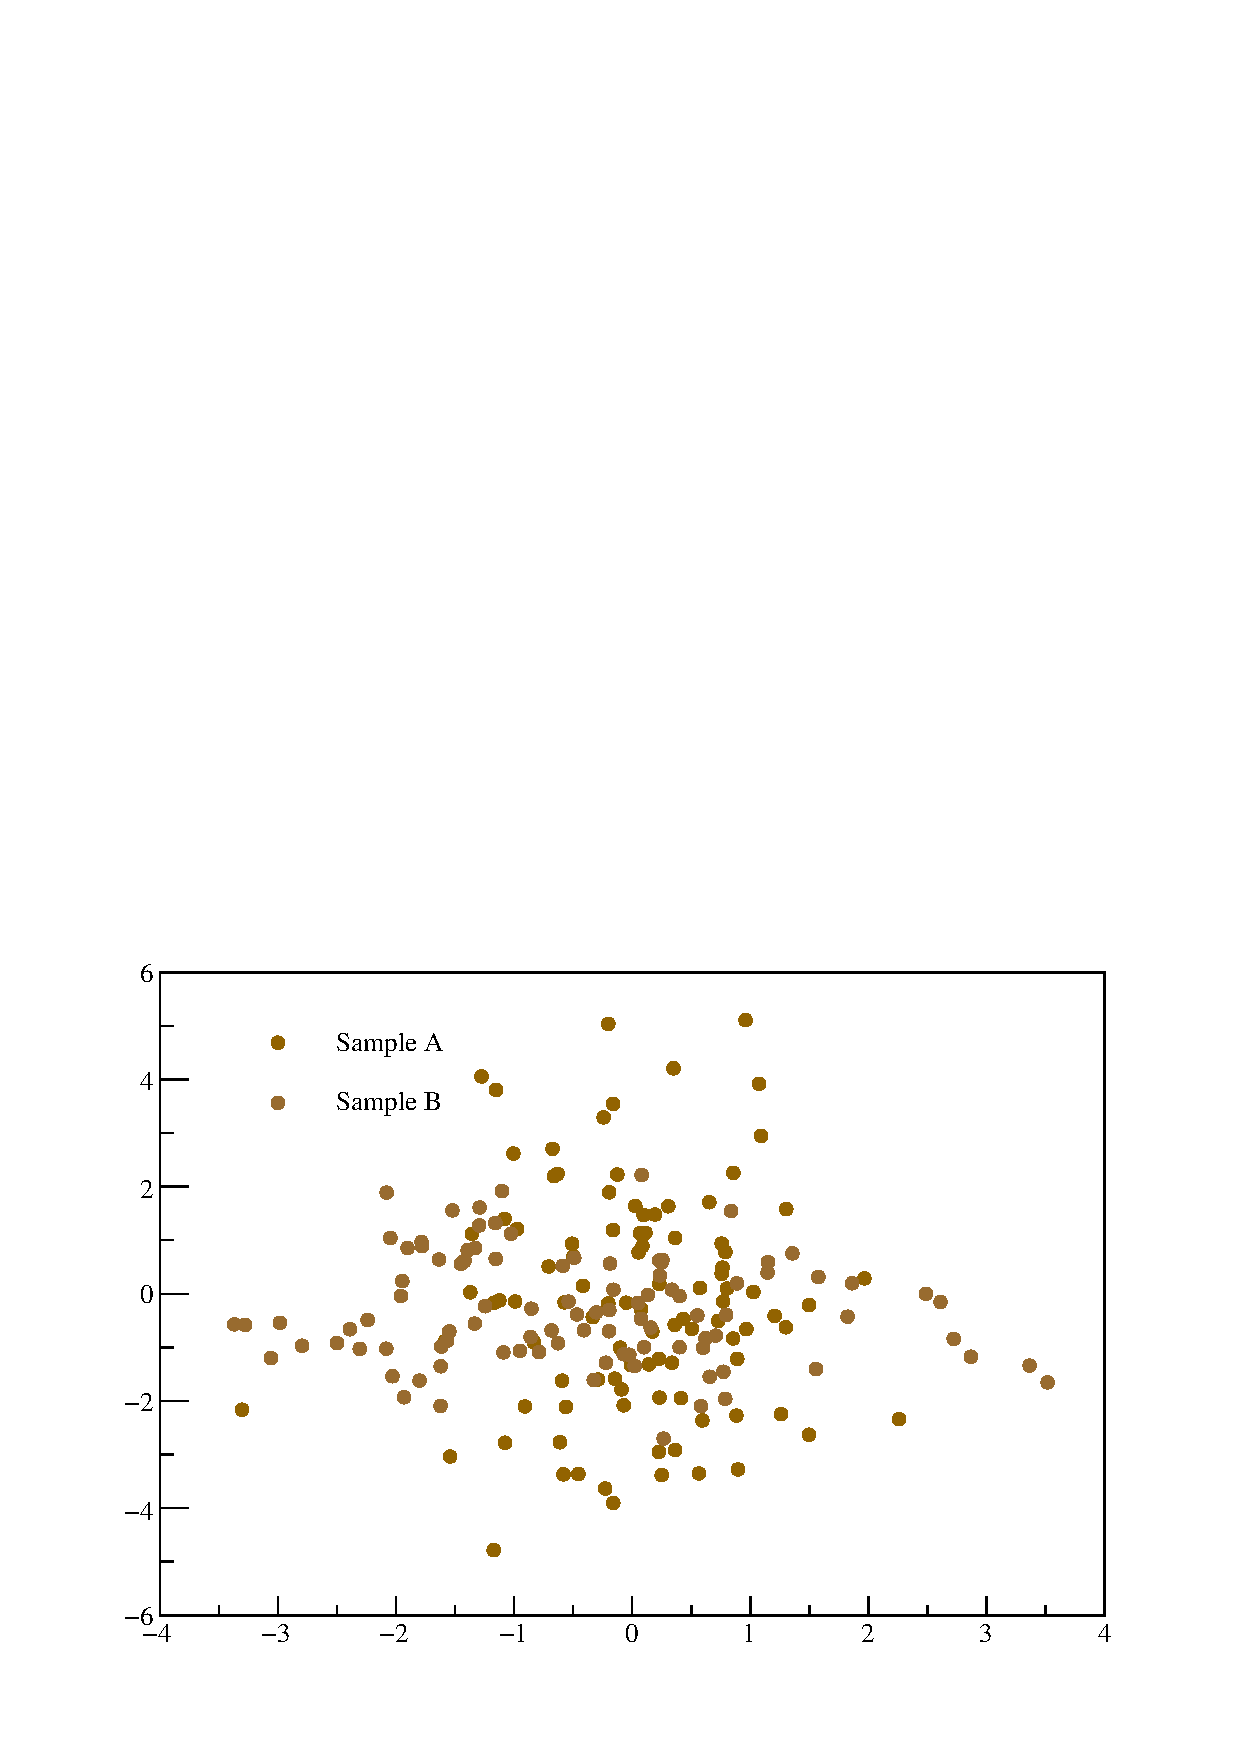
\includegraphics[width=.5\textwidth,clip]{fig/color_marker2.pdf}%
%     \label{fig_color_marker2}%
%   }
%   \subfigure[]{%
%     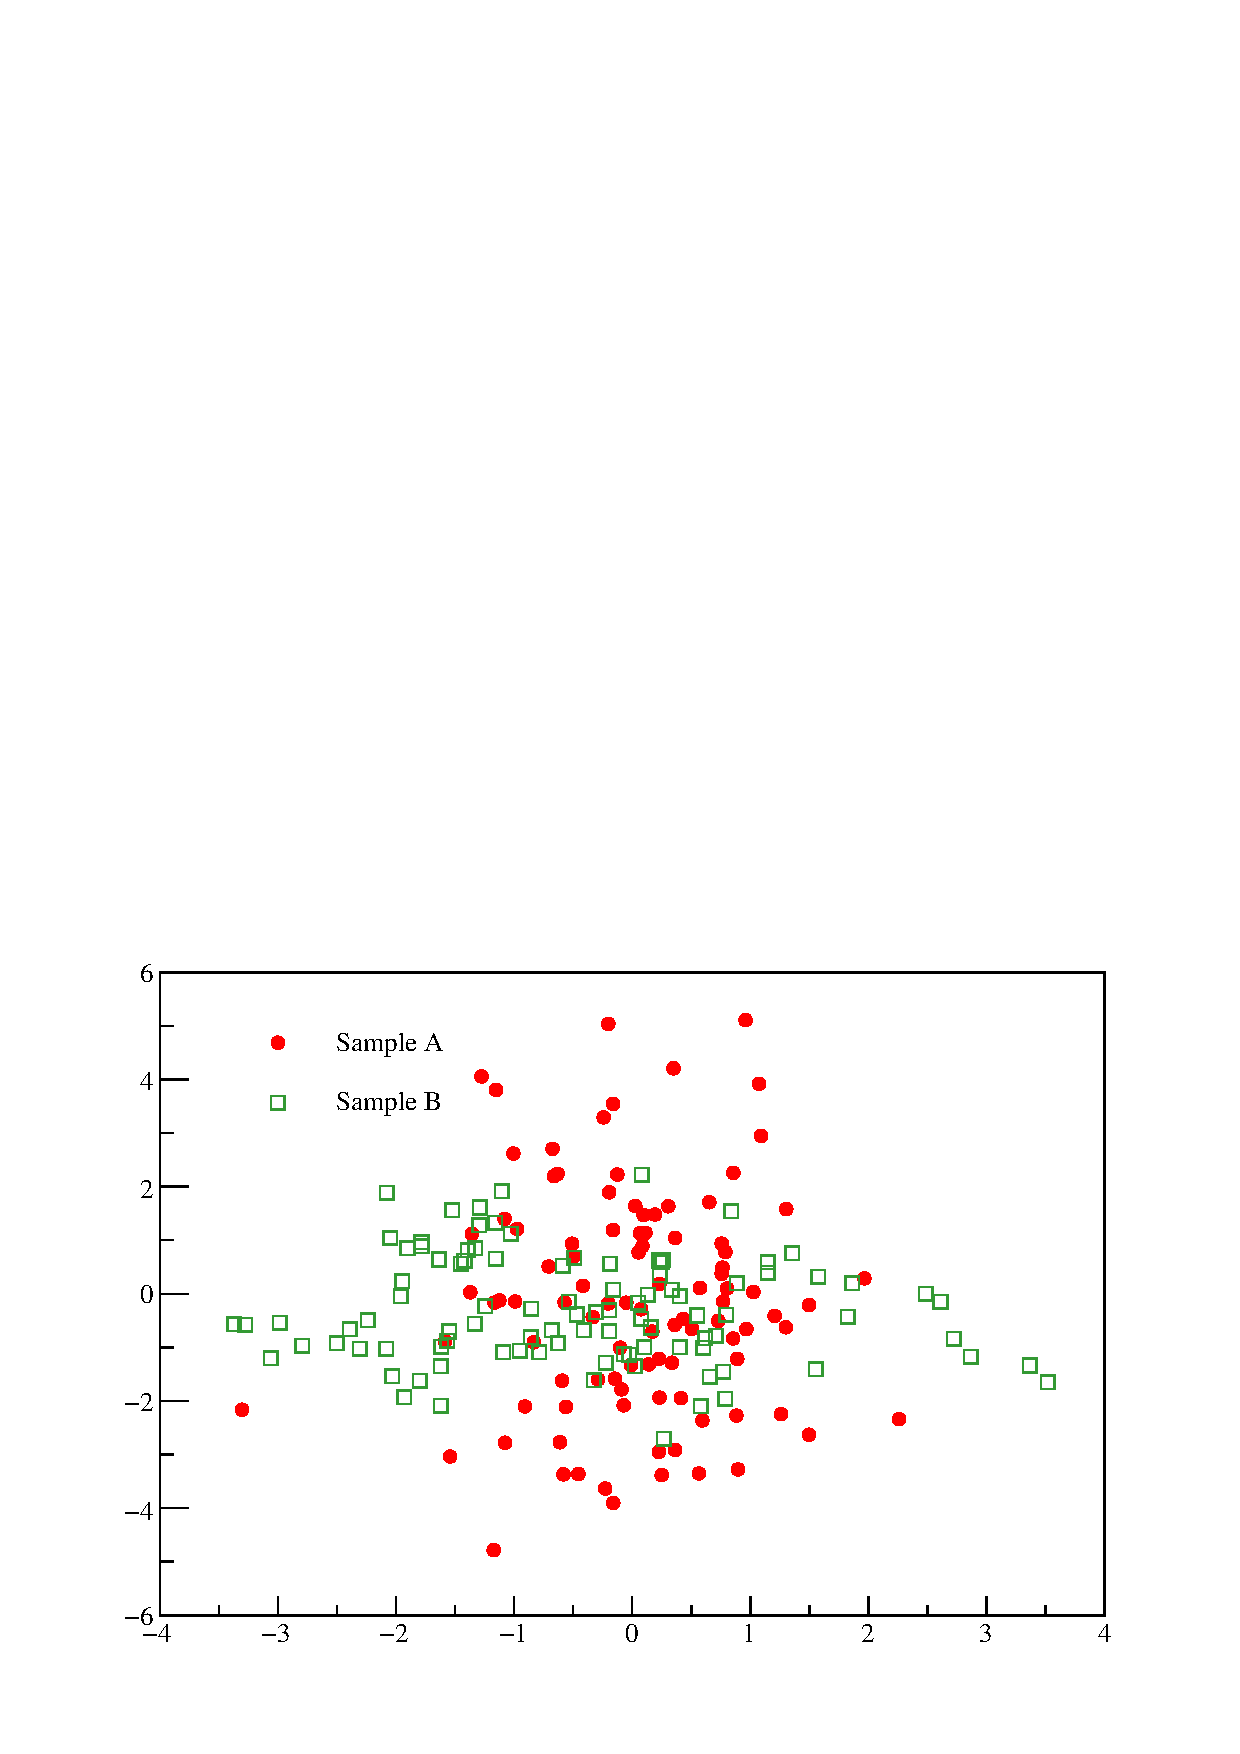
\includegraphics[width=.5\textwidth,clip]{fig/color_marker3.pdf}%
%     \label{fig_color_marker3}%
%   }%
%   \subfigure[]{%
%     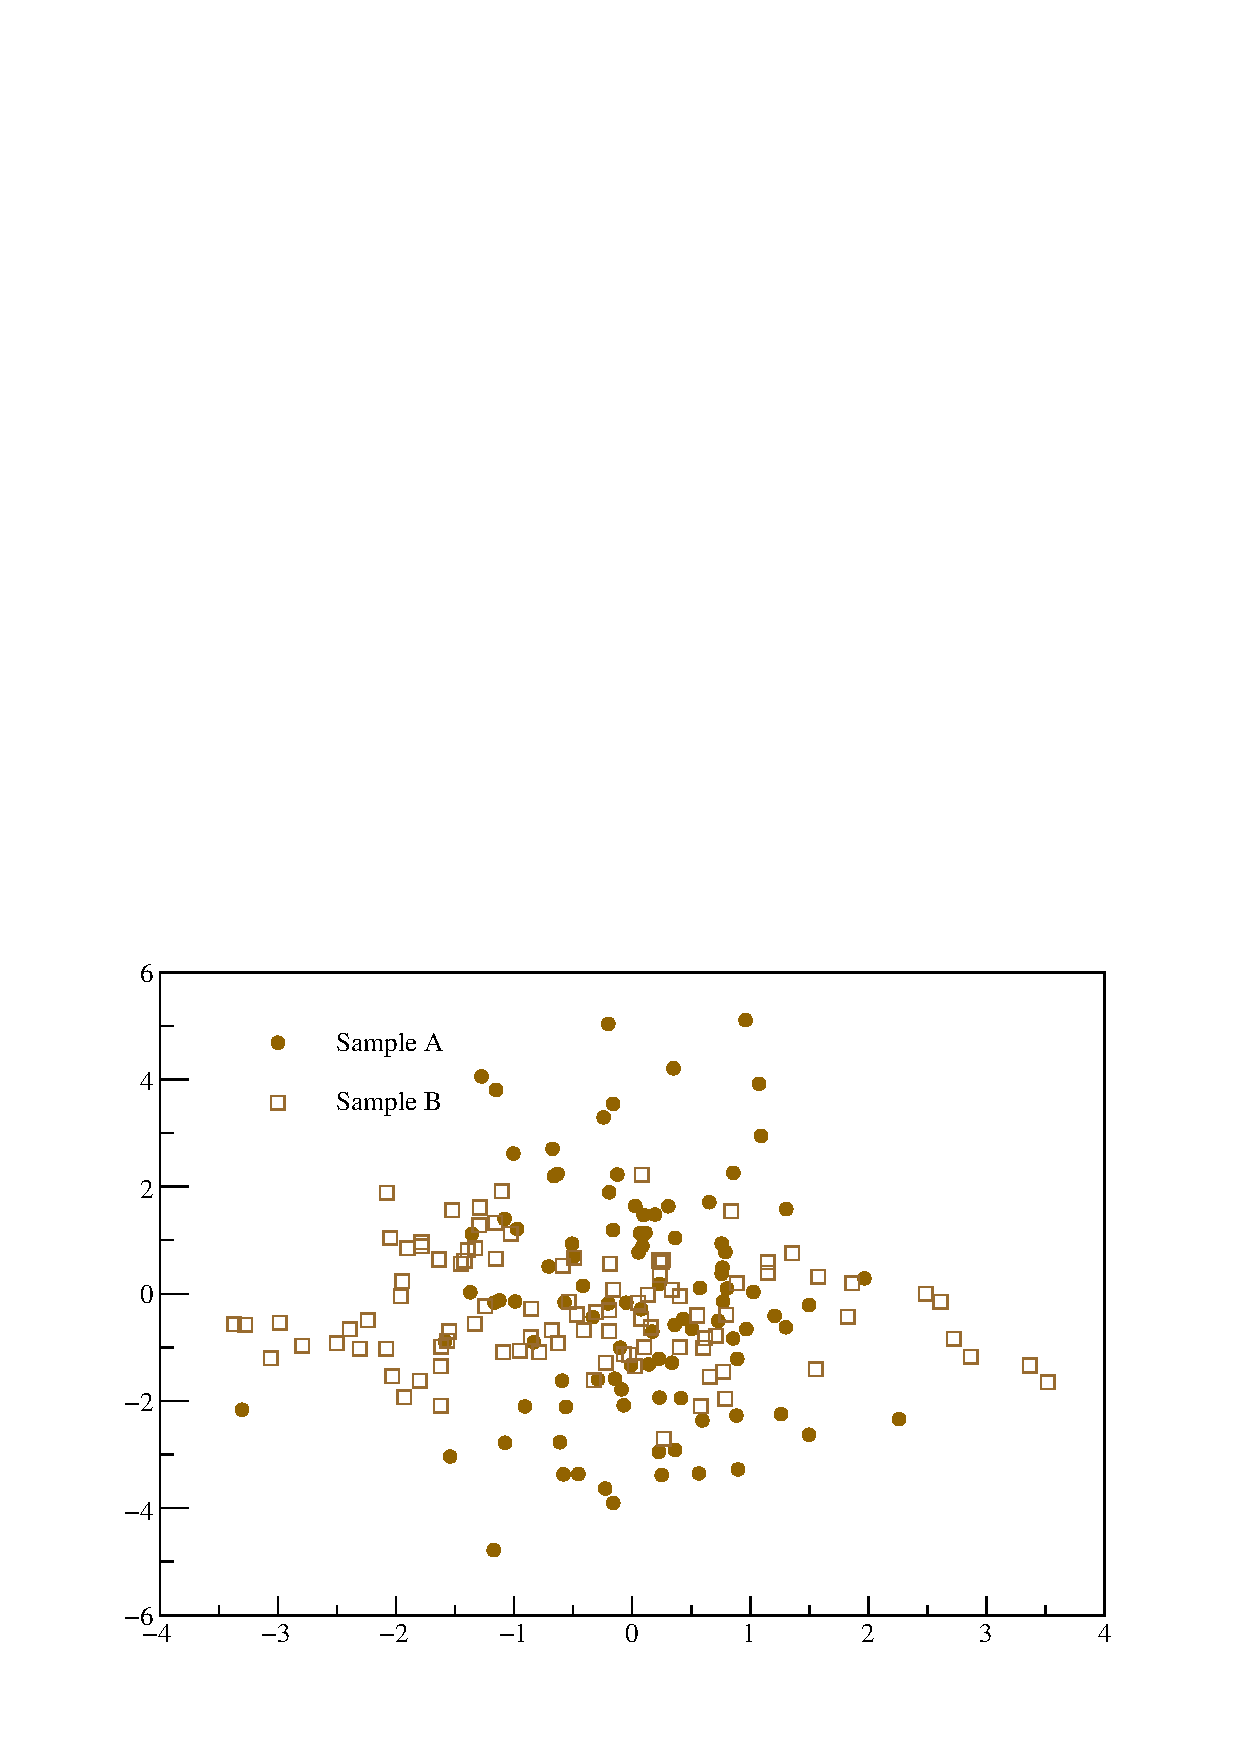
\includegraphics[width=.5\textwidth,clip]{fig/color_marker4.pdf}%
%     \label{fig_color_marker4}%
%   }
%   \caption[散布図の作図例]{散布図の作図例。(a) 色の違いしかない場合。(b) 色の違いしかない場合の見え方の例(シミュレーション)。(c) 色の違いに加えて、マーカー形状も変更した。(d) 赤と緑の区別ができなくても、マーカー形状によって区別が可能。}
% \end{figure}

\subsection{グラデーションの変更}

2次元のヒストグラムのように、線とマーカーだけでは値の増減を可視化できないものも存在します。そのようなものは色のグラデーションを使用しますが、これも注意深く選定しないと、人によっては同じ色がグラデーション中に複数回登場するように見えてしまう場合があります。

図\ref{fig_color_palette1}は虹色のグラデーションで$\sin(x)\cos(x)$を表示したものです。このグラデーションでは赤系の色と緑系の色が黄色($0.25$のあたり)を挟んで並んでいます。したがって、$0.25$ 周辺で値が変化する場合には、それが増えているのか減っているのか識別困難になります。

図\ref{fig_color_palette2}を見てみましょう。この図で左上と左下の領域が、増えているのか減っているのか区別がつくでしょうか。赤系と緑系の区別ができる人には、図\ref{fig_color_palette1}で黄緑からオレンジへの色の遷移が読み取れます。しかし、これらの色が区別できない場合、この増減は図\ref{fig_color_palette2}から読み取ることはできないのです。

% \begin{figure}
%   \centering
%   \subfigure[]{%
%     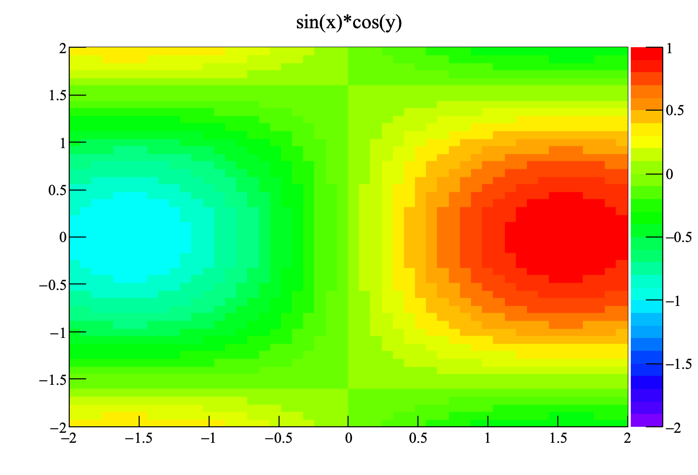
\includegraphics[width=.5\textwidth,clip]{fig/color_palette1.png}%
%     \label{fig_color_palette1}%
%   }%
%   \subfigure[]{%
%     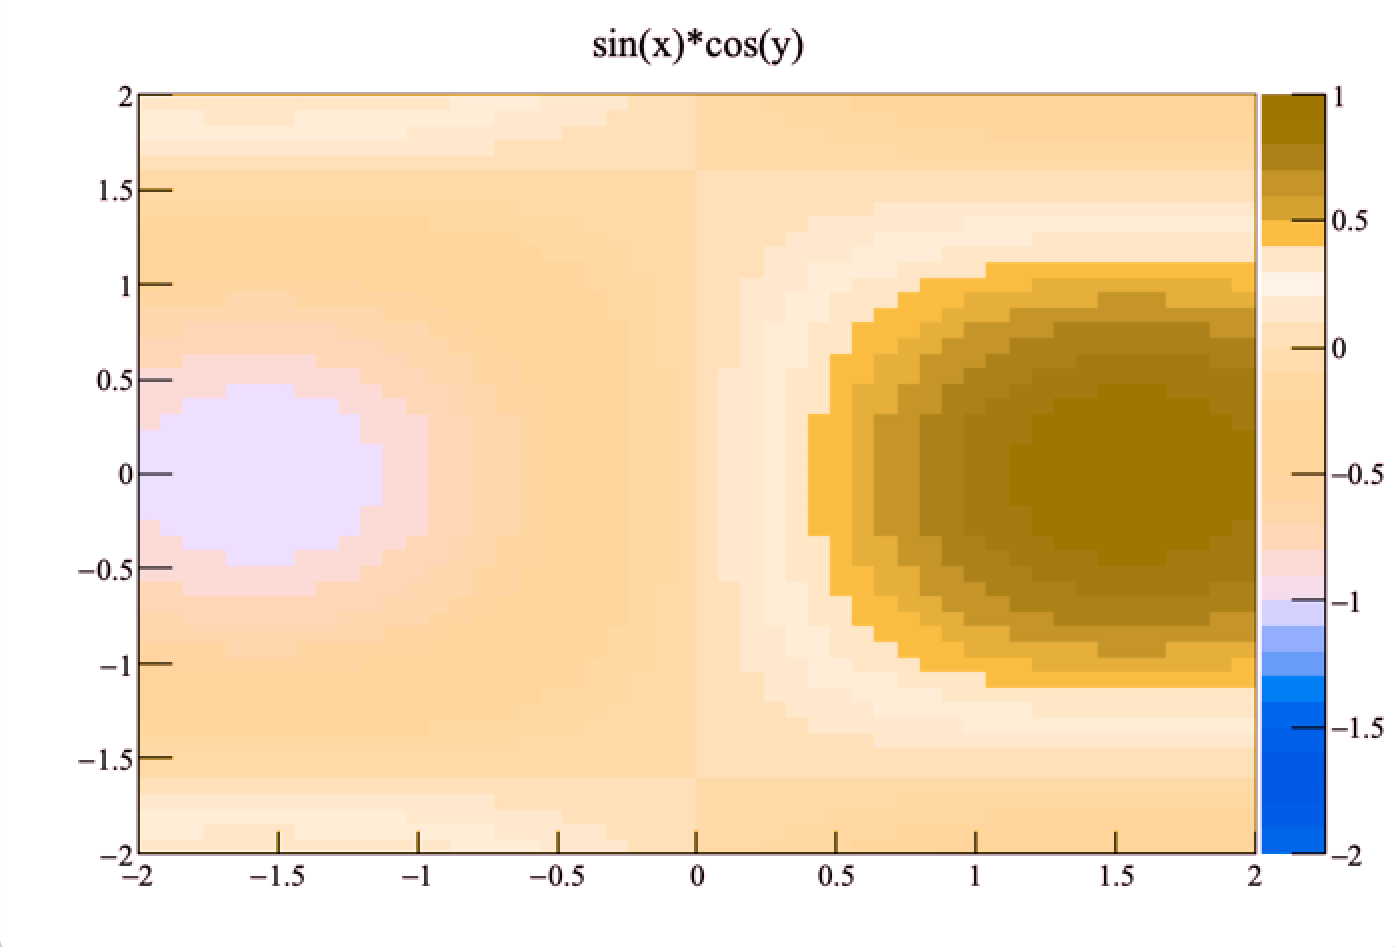
\includegraphics[width=.5\textwidth,clip]{fig/color_palette2.png}%
%     \label{fig_color_palette2}%
%   }
%   \caption[グラデーションの見え方の例]{グラデーションの見え方の例。(a) 同程度の輝度で赤系と緑系の色が出てくるグラデーションの使用例。(b) 赤系と緑系の区別がつかない場合の見え方の例(シミュレーション)。例えば左上や左下の領域が増加しているのか減少しているのか、かなり注意深く見ても識別するのが難しい。}
% \end{figure}

\subsection{色覚多様性を配慮した図になっているかの判断}

あなたが「正常」な色覚特性を持っている場合、他の人がどのように見えているかを即座に想像するのは困難です。したがって、自分の作図が誰にとっても読みやすいかを知るのは容易ではありません。しかし大原則として、「その図を白黒で印刷しても自分が正しく読み取れるか」という考え方をするのが、最も安全な判断方法だと思います。

また、色覚多様性をシミュレーションするソフトウェアも近年は無料で利用することが可能です。例えば Mac や iOS であれば「Sim Daltonism」というアプリケーションが入手可能です。図\ref{fig_color_palette2}は Mac 版の Sim Daltonism を使って見え方をシミュレーションしたものです。Windows や Android でも同様のアプリケーションがあるので、探してみてください。

\begin{itemize}
\item macOS 用の Sim Daltonism \url{https://apps.apple.com/jp/app/sim-daltonism/id693112260}
\item iOS 用の Sim Daltonism \url{https://apps.apple.com/jp/app/sim-daltonism/id1050503579}
\end{itemize}
